%! Author = charon
%! Date = 1/22/24
\section{Testumgebung}\label{sec: testumgebung}
Zur Informationsgewinnung der Funktionsweise und des Verhaltens des zu untersuchenden Binarys, muss eine Testumgebung implementiert werden.
Hierzu wurden die Antworten, die Ausgaben und die durchgeführten Aktionen des Binarys untersucht. \\
Häufig wurde die Hardware zum Testen der Netzwerkschnittstelle verwendet.
Um das Netzwerkprotokoll ortsunabhängig analysieren zu können, ohne die Hardware zur Hand zu haben,
wurden mehrere Testumgebungen implementiert.
Die konkrete Umsetzung der Testumgebungen wird in den folgenden Kapiteln erklärt.
%! Author = charon
%! Date = 2/8/24

\subsection{Testen der Netzwerkschnittstelle über die Hardware}\label{subsec: hardware}
Um möglichst einfache Fehler bei der Emulation der Umgebung zu vermeiden, wurde die Hardware verwendet.
Das \gls{iot}-Gerät verfügt über einen Ethernet-Anschluss, über den eine direkte Verbindung zur Datenübertragung
hergestellt werden kann.\\
Um möglichst genaues Feedback über das Verhalten des Binarys zu erhalten, wurde sich über \gls{ssh} mit dem Gerät verbunden.
Danach wurde das Binary, welches für das Netzwerkprotokoll verantwortlich ist, beendet und in der Aktuellen \gls{ssh}-Session neu gestartet.
Beginnt man Daten an den Port 7142 zu senden, so erhält man auf der Konsole des \gls{iot}-Geräts folgende Ausgabe.
\begin{figure}[h]
    \frame{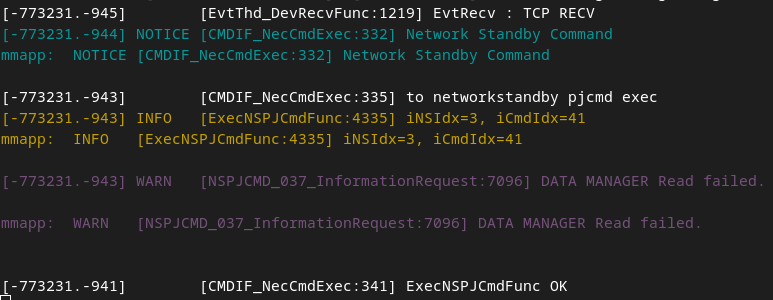
\includegraphics[width=\linewidth]{img/handler-cmd}}
    \caption{Beinhaltet die Ausgabe der Konsole nach händischem Starten des Binarys und Schicken eines Befehls an das Netzwerkprotokoll.}\label{fig:cmd-debug-info}
\end{figure}\\
Die Ausführung der Anfrage erfolgt über das Testskript \textit{binaryProt.py}~\cite{binaryProt-py}.
Das Testskript führt eine in der \texttt{main()} Funktion übergebene Funktion aus.
Es ist vorgesehen, dass alle Funktionen mit dem prefix \textit{exec} ausgeführt werden können.
Soll nur ein Befehl auf einem Gerät ausgeführt werden, so kann man die \gls{ip}-Adresse über die Konstruktoren mitgeben.
Die dokumentierten Funktionen sind bereits in menschenlesbarer Form in der Klasse \textit{Documented} enthalten.
Die Kommunikation über die Netzwerkschnittstelle erfolgt über einen Socket.
Hierzu wurde eine von Python bereitgestellte Bibliothek \textit{socket} verwendet.
Sie ermöglicht es dem Programmierer, unter Angabe einer \gls{ip}-Adresse und eines Ports, eine \gls{tcp}-Verbindung zu
einem Gerät aufzubauen.
Zur besseren Lesbarkeit wurde eine Hilfsfunktion geschrieben, welche den gesendeten Befehl in hexadezimaler Darstellung mit
einer kurzen Beschreibung der Funktionalität des Befehls in der Konsole ausgibt.
Zudem gibt das Programm die erhaltene Antwort des Befehls aus, die angibt, ob der gesendete Befehl erfolgreich auf dem
Gerät ausgeführt wurde.
Erkennbar ist die erfolgreiche Ausführung des Befehls, wenn das erste Byte der Antwort \textit{0x20}, \textit{0x21}, \textit{0x22}
oder \textit{0x23} entspricht.
Die Antworten sind ebenfalls zum Abgleich mit der Dokumentation des Protokolls~\cite{binary-prot-doc} gegenzuprüfen.
%! Author = chaorn
%! Date = 10.03.24

\begin{lstlisting}[caption={Ausgabe des implementierten Python-Skripts \textit{binaryProt.py}.
                            Es gibt den gesendeten Befehl in hexadezimaler Schreibweise,
                            sowie die \gls{ip}-Adresse des Geräts und die vom
                            Gerät gesendete Antwort aus.},label={lst:binary-prot-py-ausgabe}]
COMMAND DOCUMENTED: [base model type request] with bytes: 00 BF 00 00 01 00 C0
CHECKING IP-ADDRESS: 127.0.0.1
Sending 00 BF 00 00 01 00 C0
COMMAND SUCCESSFUL: 20 BF 01 40 10 00 FF 22 50 35 30 32 48 4C 00 00 00 00 13 FF 00 DE with checksum DE
\end{lstlisting}
Die Antworten der Befehle geben einen Hinweis darauf, dass es verschiedene Handler gibt, welche die Anfragen auf diesem Protokoll
bearbeiten.
Pahl dokumentierte die jeweiligen Handler, welche die Befehle auf dem Gerät bearbeiten, und ihre dazugehörigen Befehle
in einer Tabelle mittels des Python-Skripts~\cite{handler-table}.
Der Tabelle ist zu entnehmen, dass beim Untersuchen der Funktionen und ihrer Handler 53 dokumentierte Funktionen
vorliegen, wovon nur 26 eine valide Form besitzen.
Von diesen 26 Funktionen besitzen wiederum nur 15 einen Handler.

%! Author = charon
%! Date = 2/8/24

\subsection{Aufbau der Testumgebung mit chroot}\label{subsec: chroot}
Das Programm chroot ermöglicht das Ändern des aktuellen Wurzelverzeichnisses innerhalb eines bereits laufenden Betriebssystems.
Unter vielen Linux-Distributionen ist das Wurzelverzeichnis des Dateisystems unter dem Verzeichnispfad \textbf{/} zu finden.
Die minimale Struktur eines Linux \gls{fs}~\cite{root-fs} beinhaltet die Verzeichnisse \textit{/boot, /dev, /etc, /bin, /sbin}
und in einigen Fällen \textit{/tmp}.
Hierbei befinden sich unter \textit{/boot} Informationen zum Starten des Betriebssystems, unter \textit{/dev} Informationen zur verwendeten Hardware,
unter \textit{/etc} Konfigurationsdateien für das Betriebssystem und unter \textit{/bin} und \textit{/sbin} ausführbare Dateien (Executables). \\
Im Spezialfall des zu untersuchenden Binarys werden zum Start weitere Verzeichnisse benötigt.
Dazu gehören die Verzeichnisse \textit{/proc}~\cite{arch-procfs}, mit den darin enthaltenen Informationen zum laufenden System und Kernel,
\textit{/sys}~\cite{kernel-sysfs} mit enthaltenen Datenstrukturen, welche vom Betriebssystem verwendet werden
und \textit{/run}~\cite{runfs}, welches Systeminformationen nach dem Bootprozess des Betriebssystems enthält.
%! Author = chaorn
%! Date = 21.02.24

\begin{lstlisting}[language=bash, caption={Mounten der von chroot benötigten Verzeichnisse},label={lst:chroot-mount}]
$ sudo mount -t proc root/proc root/proc/
$ sudo mount -t sysfs root/sys root/sys/
$ sudo mount --rbind /dev root/dev/
$ sudo mount --rbind root/run root/run/
$ sudo mount --rbind /lib64 root/lib64/
$ sudo mount --rbind root/tmp root/tmp/
\end{lstlisting}
Das Mounten von \textit{/lib64} dient in diesem Script~\cite{chroot-fuzz} nur als Komfort, um nicht alle Abhängigkeiten für
\gls{afl} manuell kopieren zu müssen.
Eine Alternative dazu wäre, das \gls{afl}-Executable \texttt{afl-fuzz} statisch zu linken, damit es ohne Abhängigkeiten
ausführbar ist.
Diese Möglichkeit ist bereits im Quellcode von \gls{aflpp} eingebaut.\\
Bevor das Programm gefuzzt werden kann, muss die Umgebung mit entsprechenden Umgebungsvariablen angepasst werden.
Hierbei ist die \textit{PATH}-Variable entscheidend.
Diese ist dafür verantwortlich, dass Programme in der aktuellen \gls{bash}-Session gefunden werden.\\
Anschließend erfolgt der Wechsel in die erstellte Verzeichnisstruktur.
Die Syntax von chroot ermöglicht es, nach dem Wechsel in das neue Wurzelverzeichnis, einen \gls{bash}-Befehl auszuführen.
In diesem werden alle -- für \gls{afl} relevanten -- Umgebungsvariablen gesetzt und mit passender Instrumentierung gestartet.
%! Author = chaorn
%! Date = 21.02.24
\lstdefinestyle{chroot}{
    showstringspaces=false
}

\begin{lstlisting}[language=bash, style=chroot, caption={Wechseln in ein anderes Wurzelverzeichnis mit chroot und ausführen von AFL},label={lst:chroot-fuzzen}]
$ sudo chroot root/
    bash -c 'export AFL_DEBUG=1; export AFL_PRELOAD=./sockfuzz.so;
    export QEMU_LD_PREFIX=/;
    export PATH="/usr/gnu/bin:/usr/local/sbin:/usr/local/bin:/bin:/sbin:/usr/bin:.";
    export QT_X11_NO_MITSHM=1; export DISPLAY=:10;
    ./afl-fuzz -Q -i in -o out -t 50000 -- /app/mmapp @@'
\end{lstlisting}

%! Author = charon
%! Date = 2/8/24

\subsection{Aufbau der Testumgebung mit bwrap}\label{subsec: bwrap}
Bubblewrap ist ein Low-Level Sandboxing-Tool.
Es ermöglicht dem Nutzer, eine containerisierte Laufzeitumgebung ähnlich wie Docker, zu erstellen.
Der Unterschied zu Docker ist, dass Bubblewrap~\cite{bwrap} (oder kurz \textit{bwrap}) es ermöglicht, auch unprivilegierten Benutzern
Container -- mithilfe von Linux Kernel-User-Namespaces -- zur Verfügung zu stellen.
Der Vorteil bei der Umsetzung einer Testumgebung mit einem Container liegt darin, dass es unwahrscheinlicher ist,
das Host-System fälschlicherweise umzukonfigurieren.
Wie bereits in Abschnitt~\ref{subsec: chroot} angesprochen, müssen auch mit bwrap die entsprechenden Verzeichnisse gemountet werden,
sodass das Binary fehlerfrei funktioniert.
Das muss jedoch nicht wie bei chroot auf dem Host-System erfolgen, sondern in einer Containerumgebung.
Bwrap erstellt bei Aufruf zuerst ein leeres \gls{fs}.
Danach können alle benötigten Verzeichnisse in den Container gemountet werden~\ref{lst:bwrap-env}.
Diese Methode hat sich als die beste Methode für das hardwareunabhängige Testen erwiesen.
Mit der Isolation der Applikation über Kernel-Namespaces bietet \gls{bwrap} mit einer einfachen Syntax eine sichere Möglichkeit,
Applikationen in eine Testumgebung zu packen.
Aufgrund der Containerisierung ist es im Gegensatz zu chroot nur erschwert möglich, das eigene Betriebssystem mit dem falschen Mounten
von Verzeichnissen zu beschädigen.
Auch hat man bei der Konfiguration und Inbetriebnahme der Applikation keinen Overhead der Virtualisierung einer kompletten Plattform
wie mit Docker, was bwrap zu einem geeigneten Tool zur Implementierung einer leichtgewichtigen Testumgebung macht.
